Segmented n-type germanium detectors will be directly submerged in cryogenic liquid in GERDA Phase II. It is therefore very important to study the performance of segmented detectors in cryogenic liquid. Siegfried II, the second 18-fold segmented n-type prototype detector for GERDA Phase II (see Sec.\ref{sec:gerda:stat3}) was inserted into the Gerdanlinchen II test stand (see Sec.\ref{sec:tt:gii}) containing liquid nitrogen on April 23rd, 2008. It was kept in liquid nitrogen for about 5 months and was warmed up on September 15th, 2008. The resolution and leakage current of the core and all segments were constantly monitored. Four short cooling-down and warming-up cycles were carried out afterward to optimize the setup or to do some dedicated measurements. The leakage currents were monitored after each cooling-down. The results on the detector performance are summarized in this chapter.

\section{Experimental setup}
\label{sec:gii:setup}
The measurements were performed using the cryogenic test stand, Gerdalinchen II (GII in short). The detailed description of GII can be found in Sec.\ref{sec:tt:gii}.  Figure~\ref{fig:ii:sch} shows the setup of GII for the operation of segmented detectors in liquid nitrogen. Liquid nitrogen was filled into the dewar through the cryogenic liquid filling tube. The numbers inside the parentheses indicate the positions of eight PT100 thermal resistors. They were used to monitor the level of the liquid nitrogen. The dewar was refilled per day to keep the level of liquid nitrogen between the second and the third PT100s. The infrared shields hence were kept inside liquid nitrogen ensuring the stability of the detector working temperature. There are three mounting positions for the detectors. Only the upper and middle ones were used in the measurements.

\begin{figure}[hbtp]
\centering
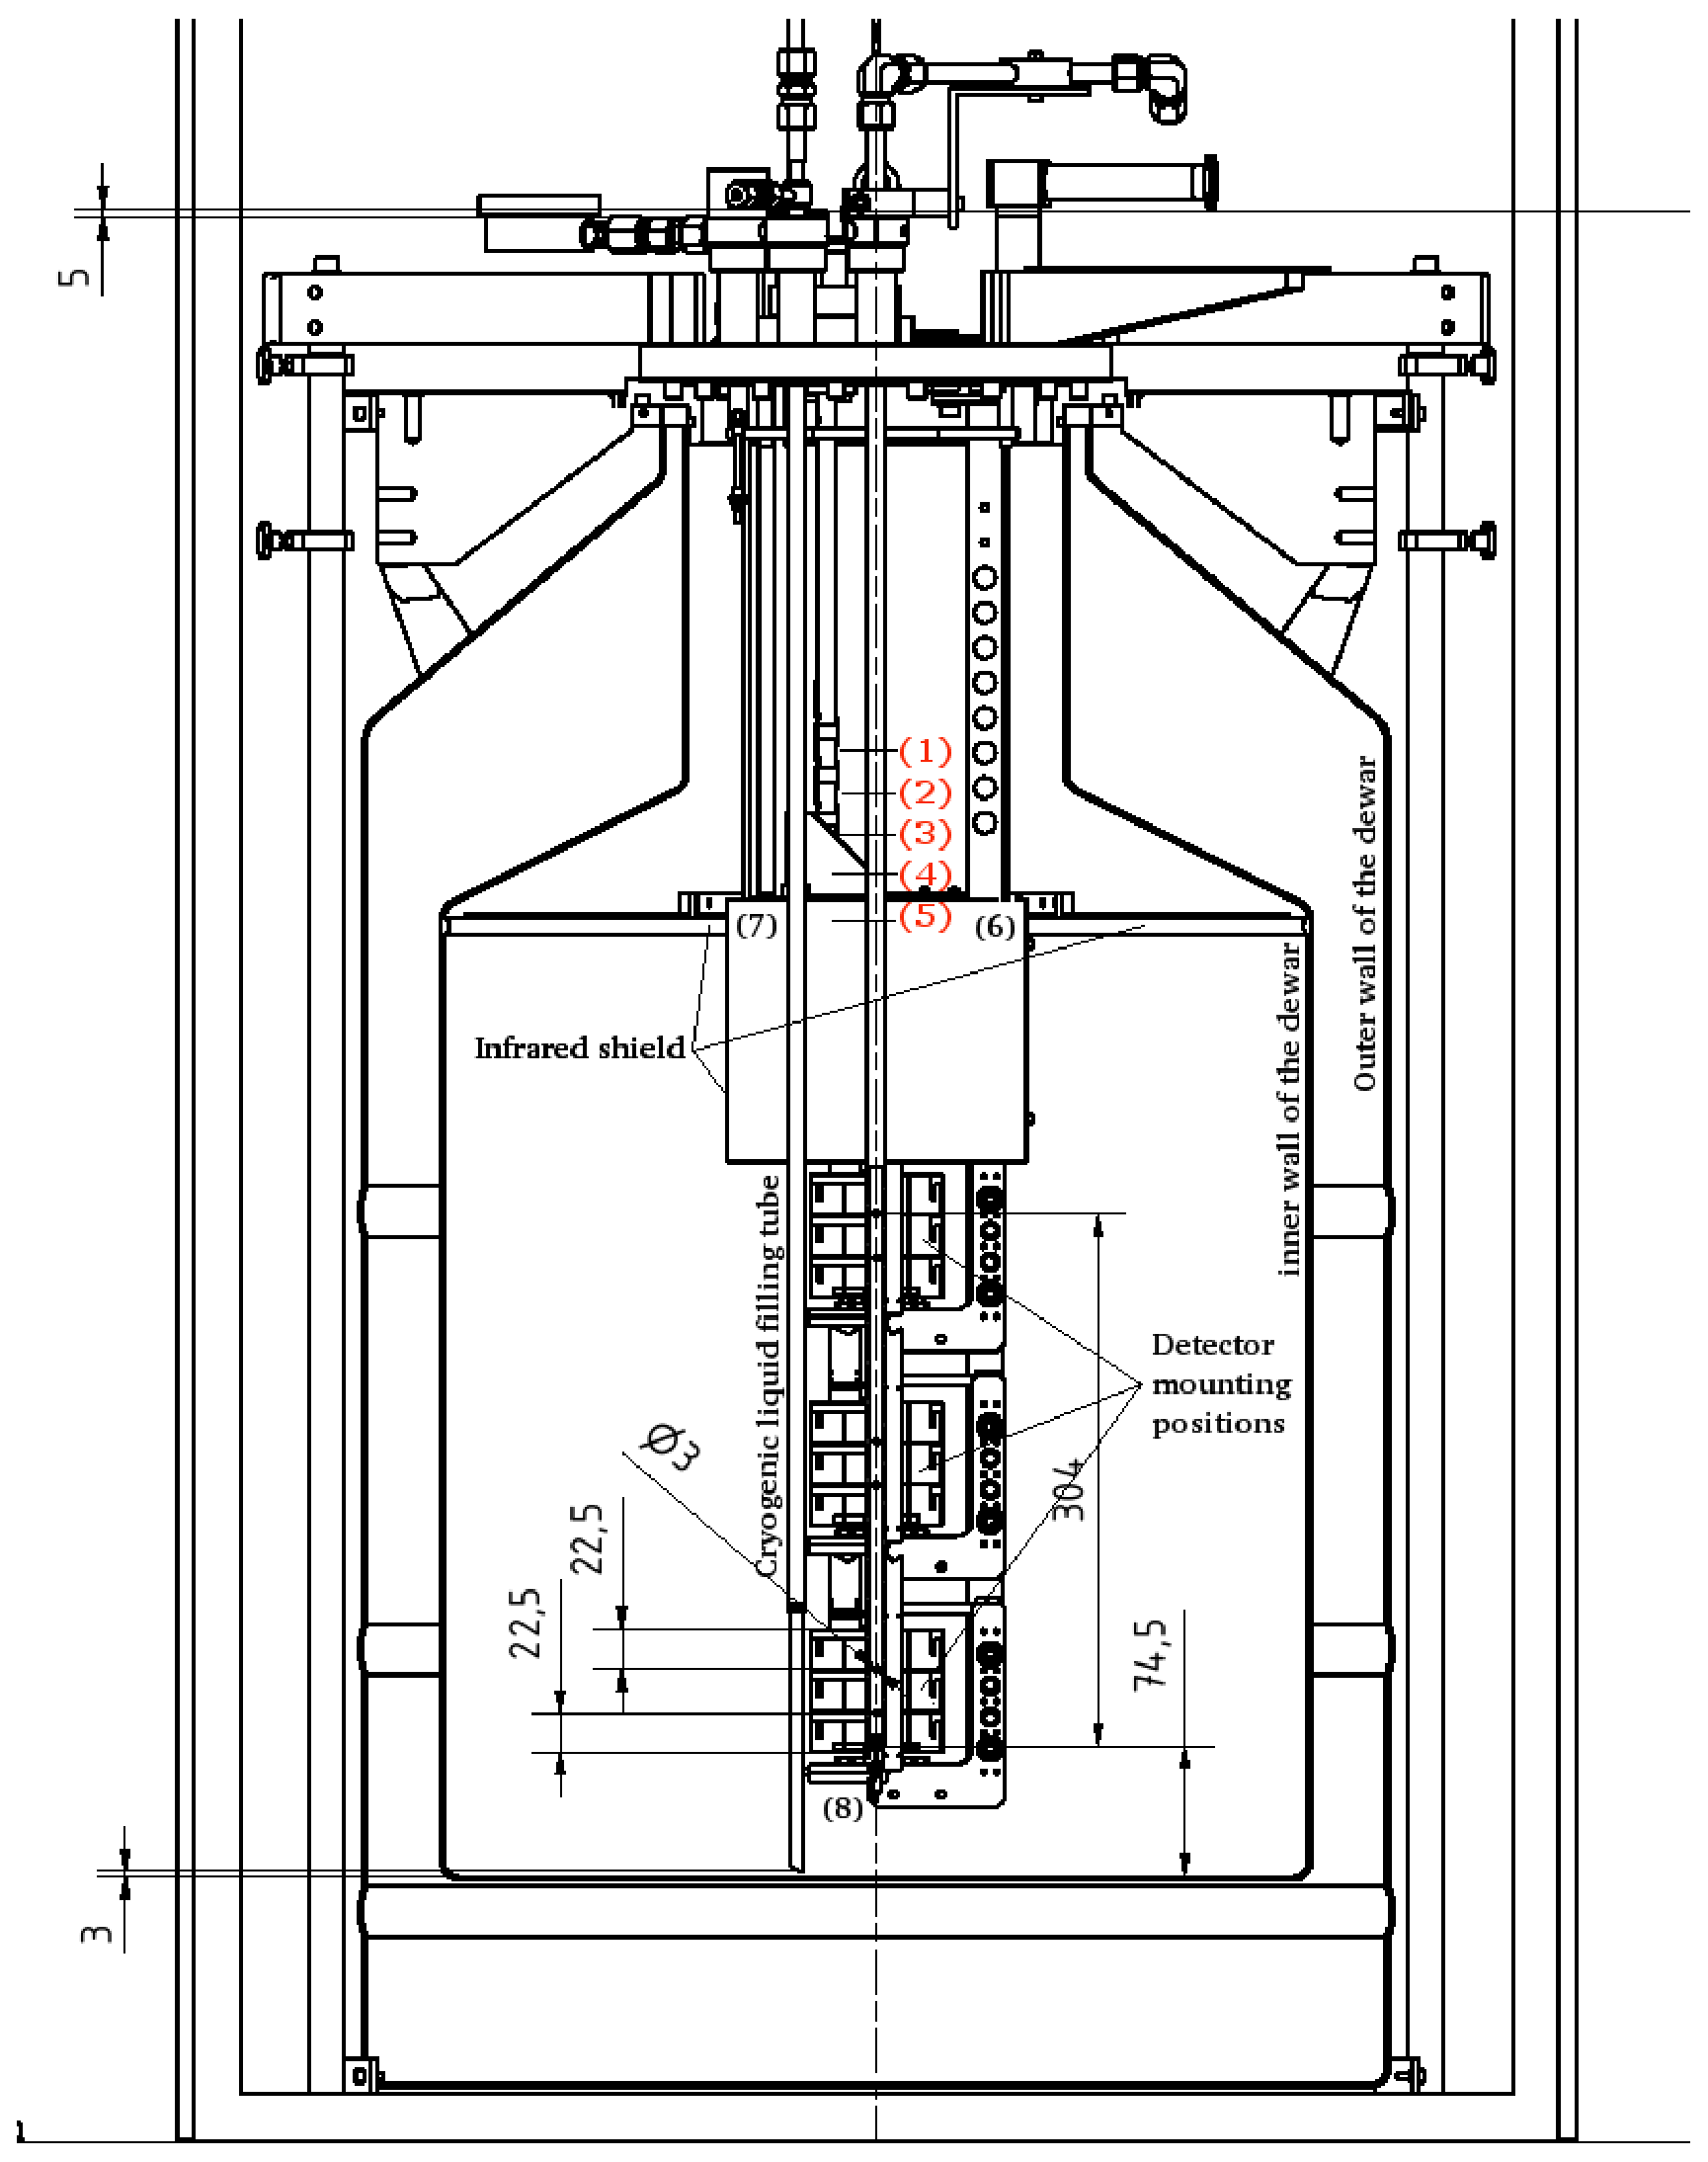
\includegraphics[width=\textwidth]{GIIscheme}
\caption{Gerdalinchen II setup for the operation of segmented detectors in liquid nitrogen.}
\label{fig:ii:sch}
\end{figure}

\section{Cooling test}
\label{sec:ii:cool}
The detector strings should be lowered into liquid argon at a moderate speed in GERDA so that the whole process can be finished in a reasonable time while the strings are kept in a stable situation. The designed submerging speed in GERDA is 10~mm/min. The temperature change of the detector during the submerging process was tested in GII with an aluminum mockup detector mounted in the highest position as shown in Fig.~\ref{fig:ii:sch}. The filling speed of liquid nitrogen was tuned to be about 10~mm/min. The tempareture profile of the mockup detector was monitored using three PT100 thermal resisters mounted on the top, bottom and in the middle of the mockup. Figure~\ref{fig:ii:temp} shows the tempareture changes of the mockup detector during the filling of GII. The positions of the 1$^{\text{st}}$ and the 8$^{\text{th}}$ thermal sensor are indicated in Fig.~\ref{fig:ii:sch}. Curves labled ``Top'', ``Middle'' and ``Bottom'' show the tempareture changes of the mockup detector. The largest tempareture difference between the top and bottom of the mockup detector is about 130~$^{\circ}$C. However, this large difference only lasted about 3 minutes. In most of the time the tempareture difference was very small.
\begin{figure}[htbp]
\centering
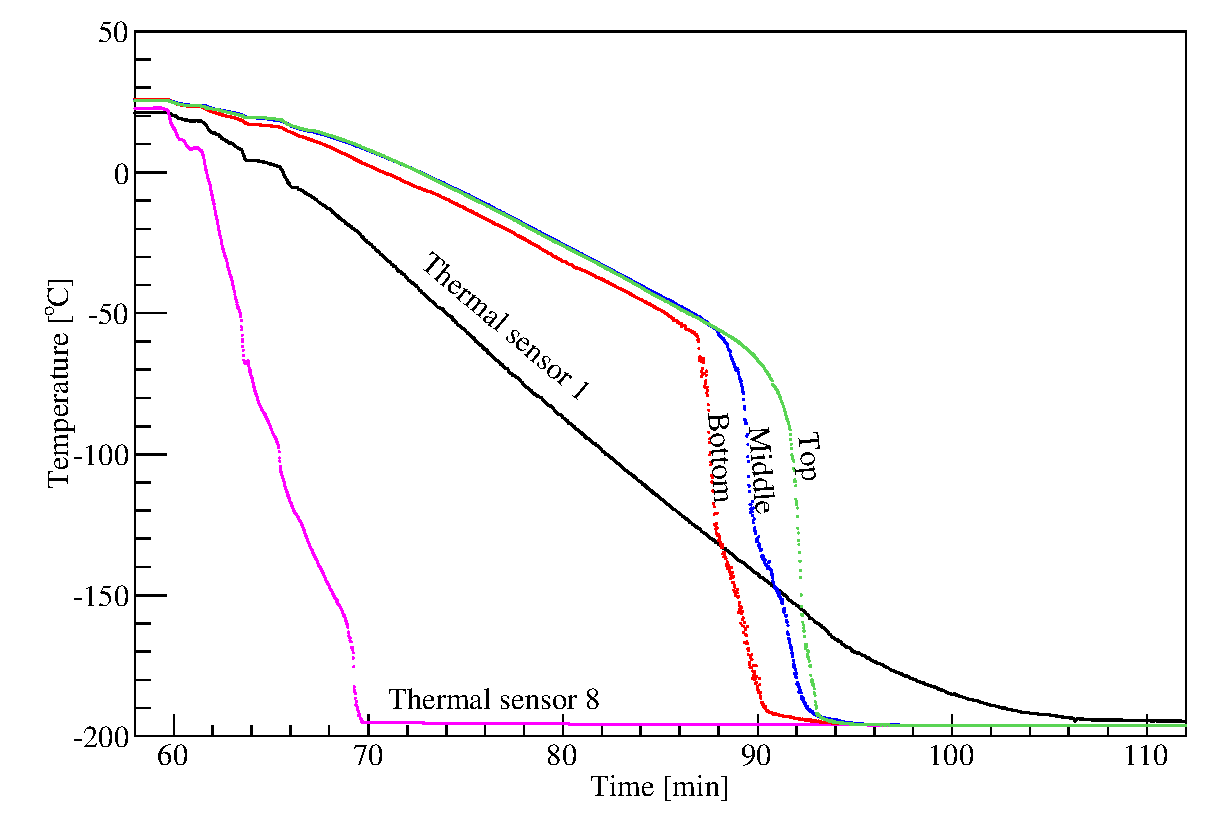
\includegraphics[width=0.8\textwidth]{temp}
\caption{Temperature profile of mockup detector during cooling down process. GII was filled with liquid nitrogen at the speed of 10~mm/min. Positions of the 1$^{\text{st}}$ and the 8$^{\text{th}}$ thermal sensor are indicated in Fig.~\ref{fig:ii:sch}. Curves labled ``Top'', ``Middle'' and ``Bottom'' show the tempareture changes of the mockup detector.}
\label{fig:ii:temp}
\end{figure}

\section{History of resolution}
\label{sec:ii:sigma}
Siegfried II was mounted at the hightest detector mounting position in GII after a detailed cooling procedure was worked out. It was cooled down on April 23$^{\text{rd}}$, 2008. The core and segment resolutions of Siegfried II were constantly monitored during the 140 days of operation. The variation of the resolution (FWHM) at 1332~keV is shown for the core channel in Fig.~\ref{fig:ii:fwhm_core} and for all 18 segments in Fig.~\ref{fig:ii:fwhm_segs}.
\begin{figure}[hbtp]
\centering
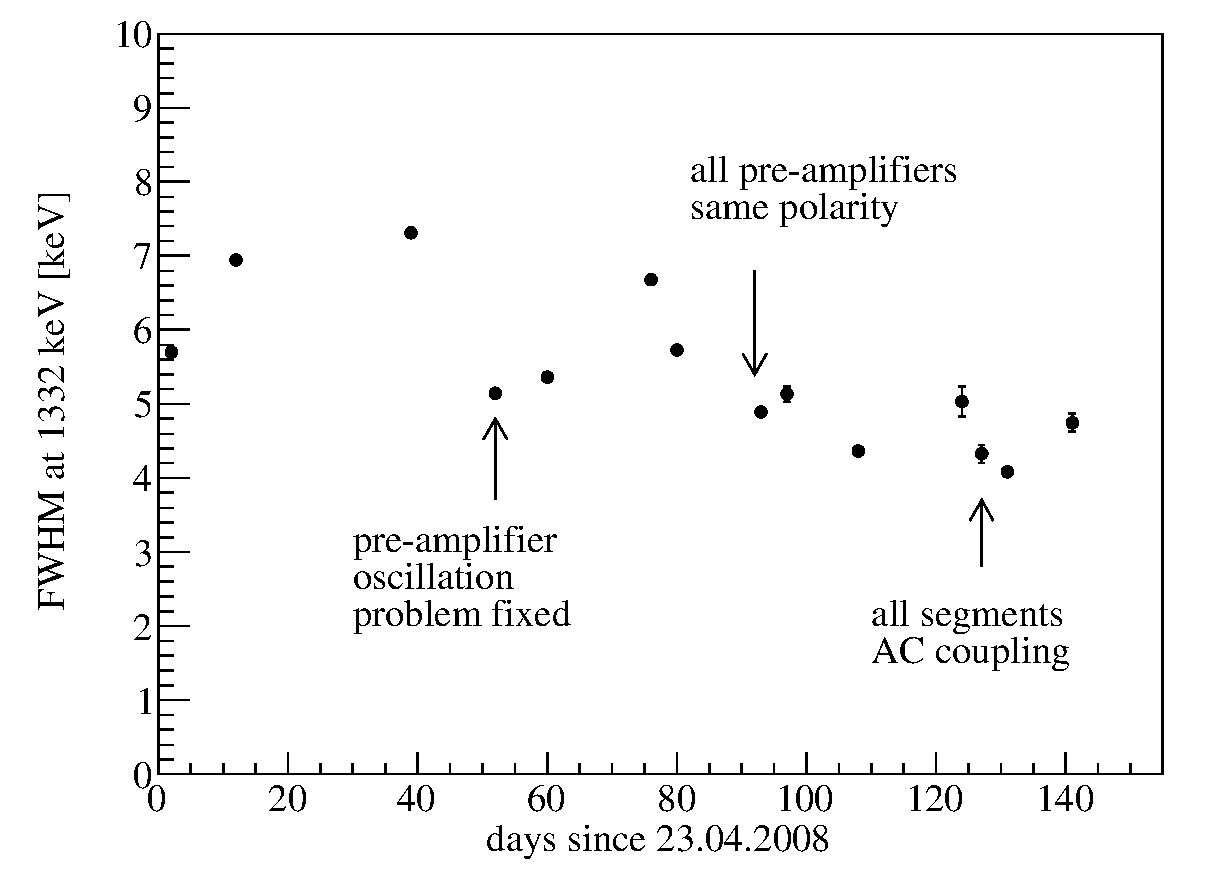
\includegraphics[width=0.6\textwidth]{fwhm_versus_time_core}
\caption{History of the core resolution of Siegfried II during 140 days of operation.}
\label{fig:ii:fwhm_core}
\end{figure}

\begin{sidewaysfigure}[tphb]
\centering
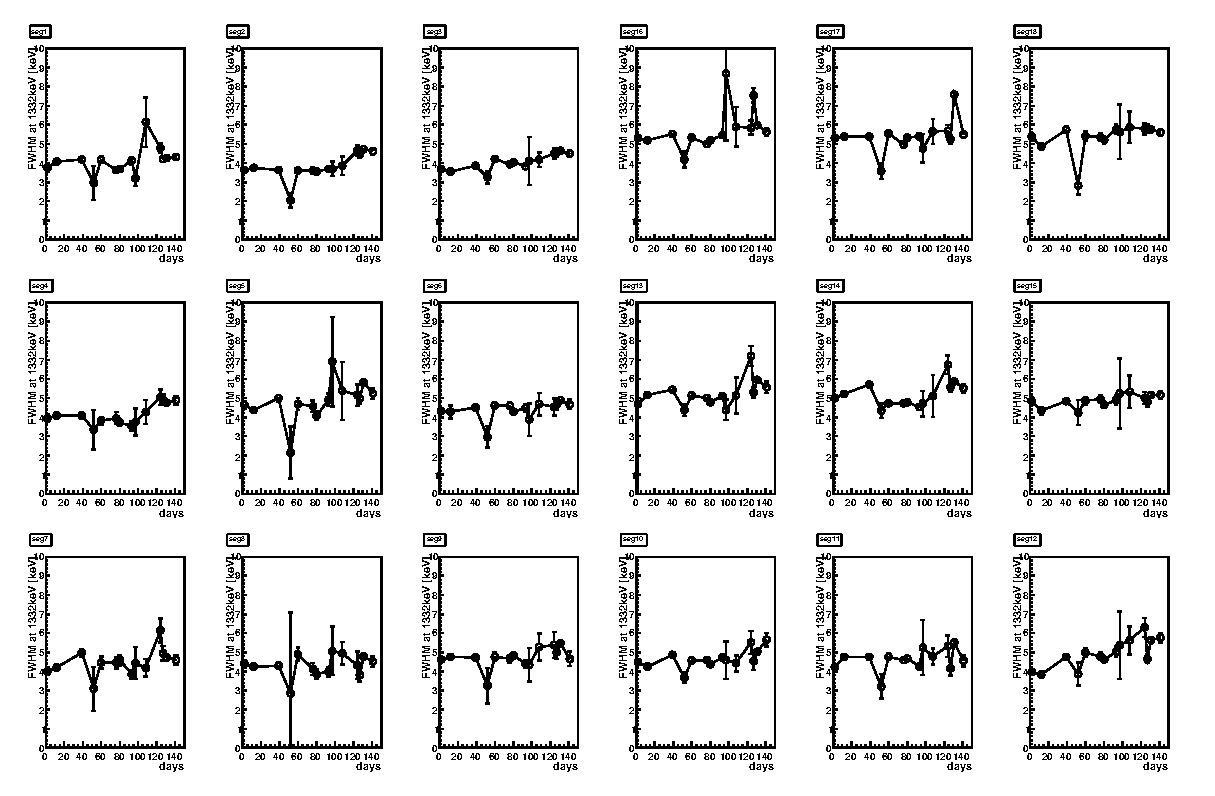
\includegraphics{fwhm_versus_time_segments}
\caption{History of the segment resolutions of Siegfried II during 140 days of operation.}
\label{fig:ii:fwhm_segs}
\end{sidewaysfigure}

During the first month of operation, all preamplifiers were oscillating if all 19 channels were read out simultaneously. The oscillation was due to the bad grounding scheme of the copper boxes holding and shielding the preamplifiers (see Fig.~\ref{fig:tt:gefb}). The problem was fixed by adding an extra copper plate inside the box, which serves as the commond ground for all preamplifiers. Afterwards, all preamps could be read out simultaneously
and the core resolution was slightly improved as well.

The second problem which affected the core resolution was related to the pulse polarity of the preamplifiers. Three preamplifiers (segments 3, 15 and 17) had negative signal pulse while the rest had positive pulse. Though the polarity of these three preamplifiers were corrected in the DAQ system, certain cross talks were observed between these three preamplifiers and the core preamplifier. Take the 1332~keV photon line as an example, for events with the photon energy deposited inside any of these three segments the energy measured by the core preamplifer is about 2~keV smaller than the measured core energy in those events with the same photon energy deposited inside any other segments. These three preamplifiers were then replaced, resulting in some improvement in the core resolution as indicated in Fig.~\ref{fig:ii:fwhm_core}.

In order to obtain a better defined potential of segments, all segment preamplifiers were modified from DC to AC coupling ten days before the first warming up, using 1~G$\Omega$ resistors and 2.2~nF capacitors. This improved slightly the core resolution, but not those of the segments.


\section{Leakage current}
\label{sec:ii:current}
The leakage current of Siegfried II at 2000~V was constantly monitored during the first 140 days of operation. Two measurement methods were used: (a) direct measurement with a peco-amparemeter and (b) indirect measurement by comparing the baseline movement at 0~V and 2000~V. The results from these two different measurements are both shown in Fig.~\ref{fig:ii:lc}. The leakage current stayed constantly around 20~pA except one measurement which was probably performed incorrectly.

\begin{figure}[htbp]
\centering
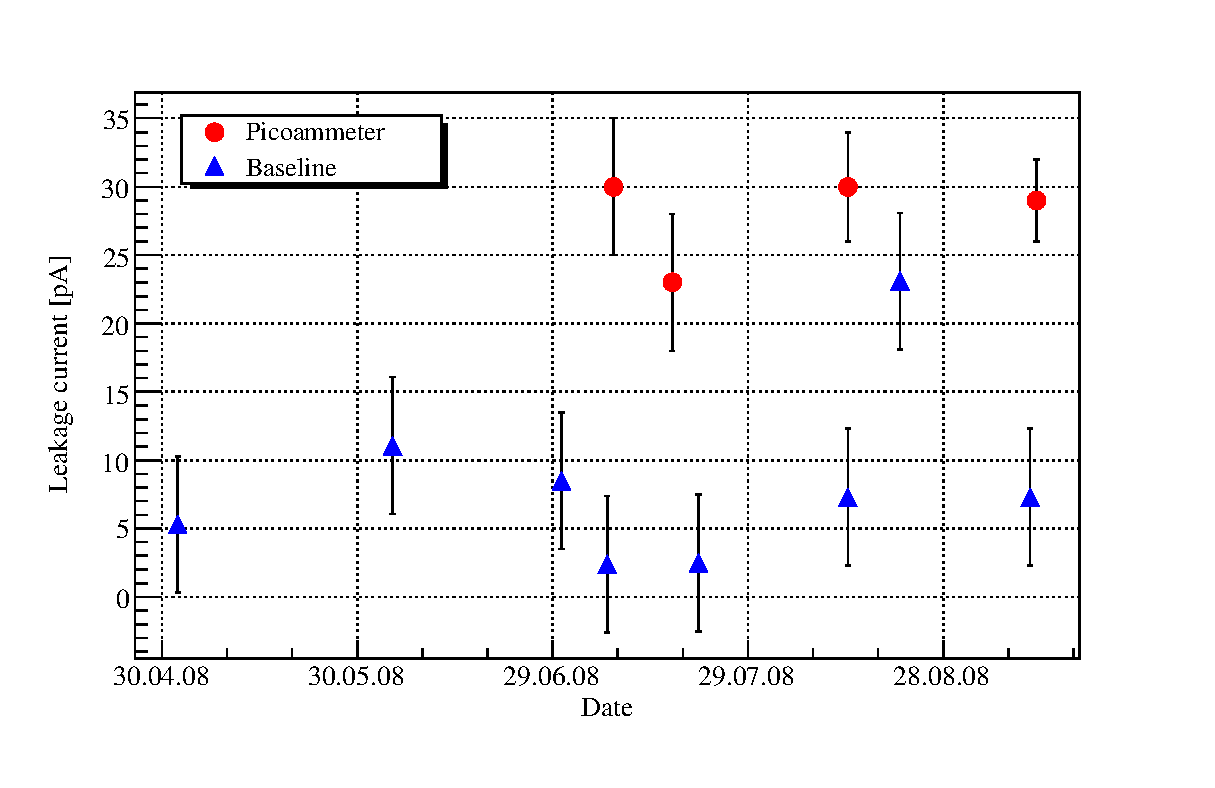
\includegraphics[width=0.6\textwidth, clip]{LC}
\caption{Leakage current of Siegfried II at 2000~V. Two different measurement methods were used. The first was to use a peco-amparemeter to directly measure the leakage current at 2000~V. The second was to compare the baselines of pulses at 0~V and 2000~V.}
\label{fig:ii:lc}
\end{figure}

Siegfried I was mounted to the middle detector mounting position in GII after the first warming-up of Siegfried II. Aferwards, four cooling-down and warming-up cycle were performed. Leakage currents of Siegfried I and II at operation voltage after each cooling-down were measured as shown in Fig.~\ref{fig:ii:lcs1} and \ref{fig:ii:lcs2}, respectively. The immediate measurements after each cooling-down showed dramatic increase of the leakage current. However, the leakage current kept dropping until reaching a constant value within around 40 minutes after the cooling-down. The measurements after that showed no increase of leakage current. This indicates some increase of the capacitance of the contacts between the detector surfaces and the signal cables.

\begin{figure}[htbp]
\centering
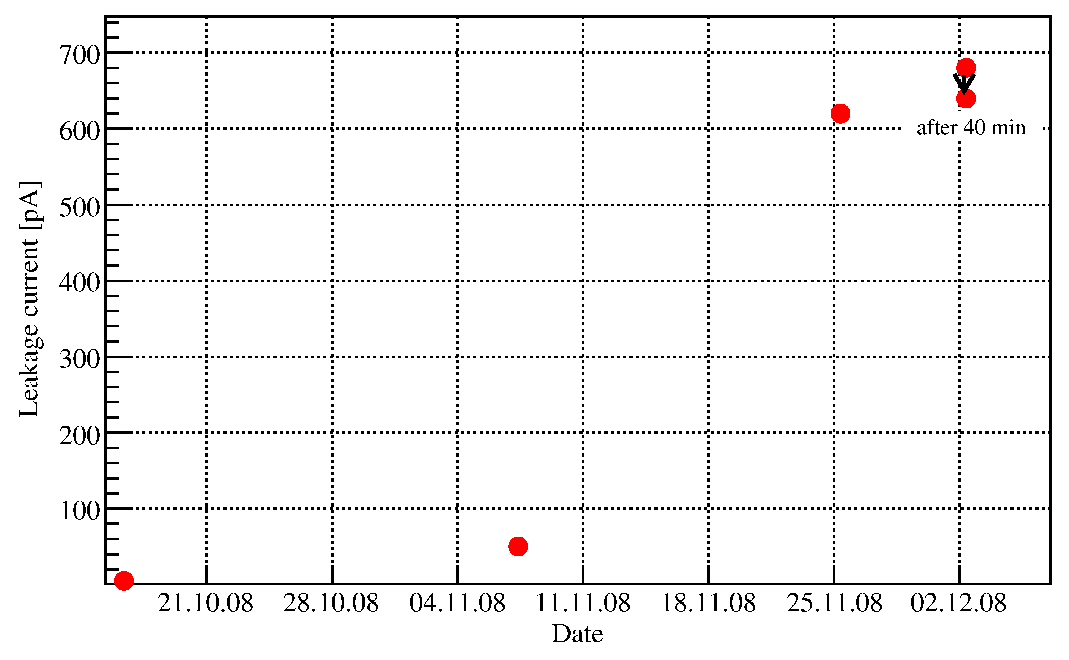
\includegraphics[width=0.6\textwidth]{LCs1}
\caption{Leakage current of Siegfried I at 3000~V right after each cooling-down. The current was directly measured using a peco-amparemeter.}
\label{fig:ii:lcs1}
\end{figure}

\begin{figure}[htbp]
\centering
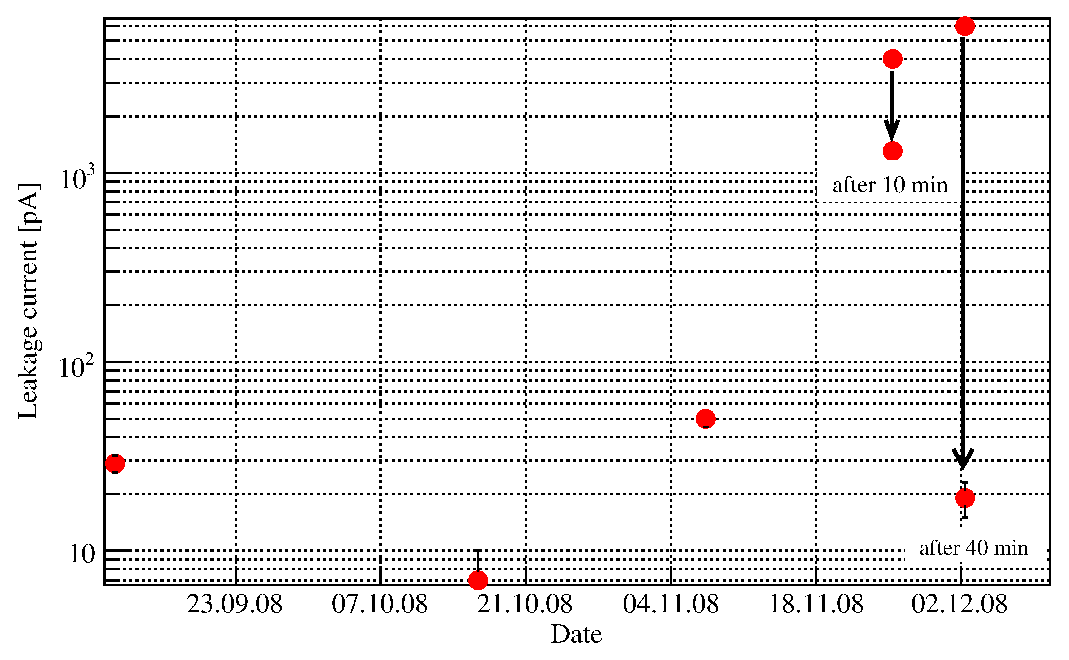
\includegraphics[width=0.6\textwidth, clip]{LCs2}
\caption{Leakage current of Siegfried II at 2000~V after each cooling-down. The current was directly measured using a peco-amparemeter.}
\label{fig:ii:lcs2}
\end{figure}

% \section{Capacitance measurement}
% \label{sec:ii:c}

% \section{Cross talk}
% \label{sec:ii:xtalk}
% with siegfried-II mounted.  The HV cable was connected through the HV feedthrough built on the top flange.  The shield of the HV cable was connected to the top flange.  Under the flange (thus inside the dewar) non-shielded Habia cable (?) was used for both the HV cable and the signal cables for the 18 segments.  A 2.2~nF capacitor and 1~G$\Omega$ resistor were used for the HV filter.  Another 2.2~nF capacitor was used for the core AC coupling. The two capacitors and the resistor were positioned right below the top flange, thus not inside the liquid Nitrogen and only in the gas Nitrogen enviroument.

\section{Negative pulse}
\label{sec:ii:npulse}
The preamplifiers and DAQ system were configured such that all the channels had positive polarity, \textit{i.e.}, the signals were positive pulses. About 10\% of the events were found to have negative pulses in some of the segments. Figure~\ref{fig:ii:npul} shows a typic negtive pulse event. It was a single-segment event, namely, there was only one segment (segment 2) having energy deposited. Segment 2 had a positive pulse. Transient pulses were induced in its neighboring segments 1 and 3. It is shown clearly that the baseline of the pulse in segment 3 dropped, which made it look like a negtive pulse.

\begin{sidewaysfigure}[htbp]
\centering
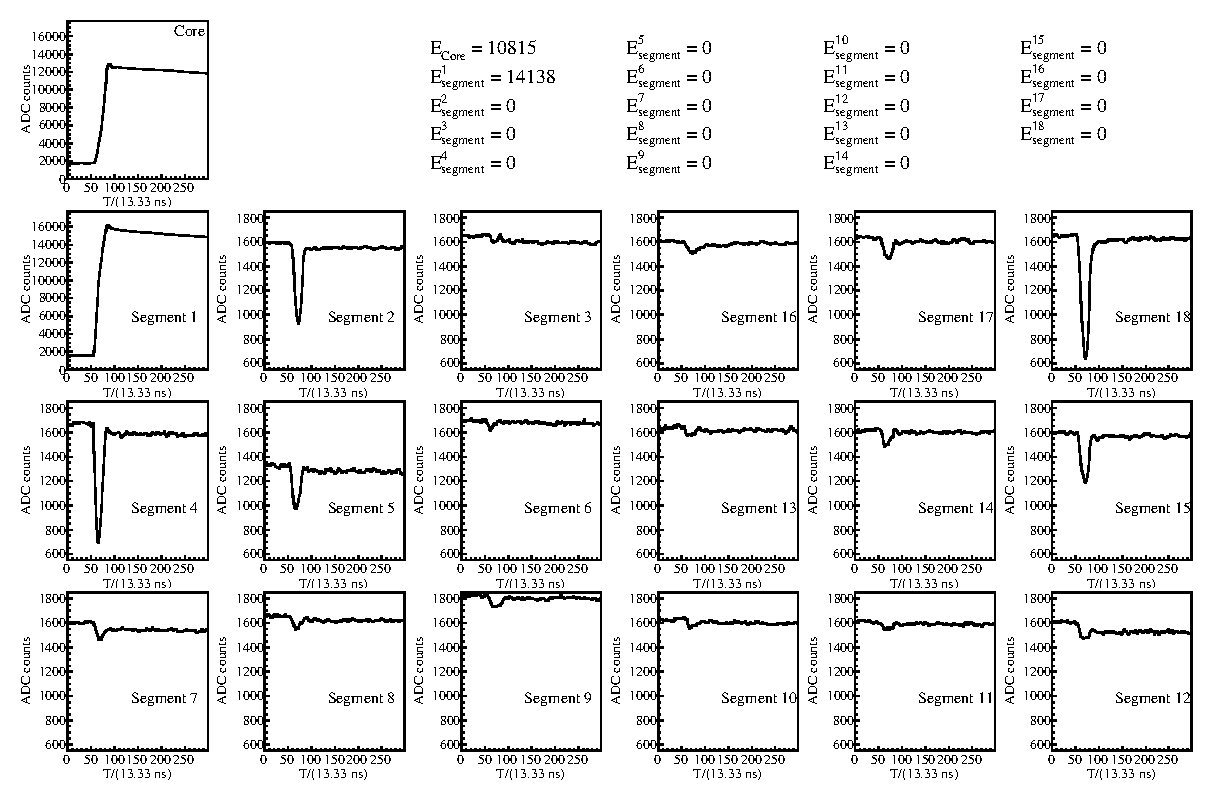
\includegraphics{npul}
\caption{An event showing negative pulse in one segment.}
\label{fig:ii:npul}
\end{sidewaysfigure}

\subsection{Selection of negtive pulse events}
\label{sec:ii:frac}
The sum of energies from all the segments, $\sum E_{\text{segment}}$, (including those with negtive pulses. They gave negative values.) agrees with the core energy, $E_{\text{core}}$, within the resolution. However, since the DAQ system estimated the energy of a negative pulse to be zero (as shown in the top right part of Fig.~\ref{fig:ii:npul}), the sum of the segment energies as calculated by DAQ, $\sum E^{\text{DAQ}}_{\text{segment}}$, was larger than $E_{\text{core}}$. By comparing  $\sum E^{\text{DAQ}}_{\text{segment}}$ and $E_{\text{core}}$, negative pulse events were identified and selected.

Figure~\ref{fig:ii:sEnegPulse} shows $\sum E^{\text{DAQ}}_{\text{segment}}$ versus $E_{\text{core}}$ of a data sample collected with an $^{228}$Th source mounted inside GII on top of Siegfried II. The two solid lines in the plot indicate the 20$\sigma$ range of the core energy. Points above the upper solid line correspond to the negative pulse events because they have $\sum E^{\text{DAQ}}_{\text{segment}} \gg E_{\text{core}}$. There is also a very small fraction of events with$\sum E^{\text{DAQ}}_{\text{segment}} < E_{\text{core}}$. This is due to the noise or pile-up\footnote{Two pulses are too close to each other in time for DAQ to get a correct estimation of energy.} effect. The fraction of negative pulse events is about 10\%.

\begin{figure}[tphb]
\centering
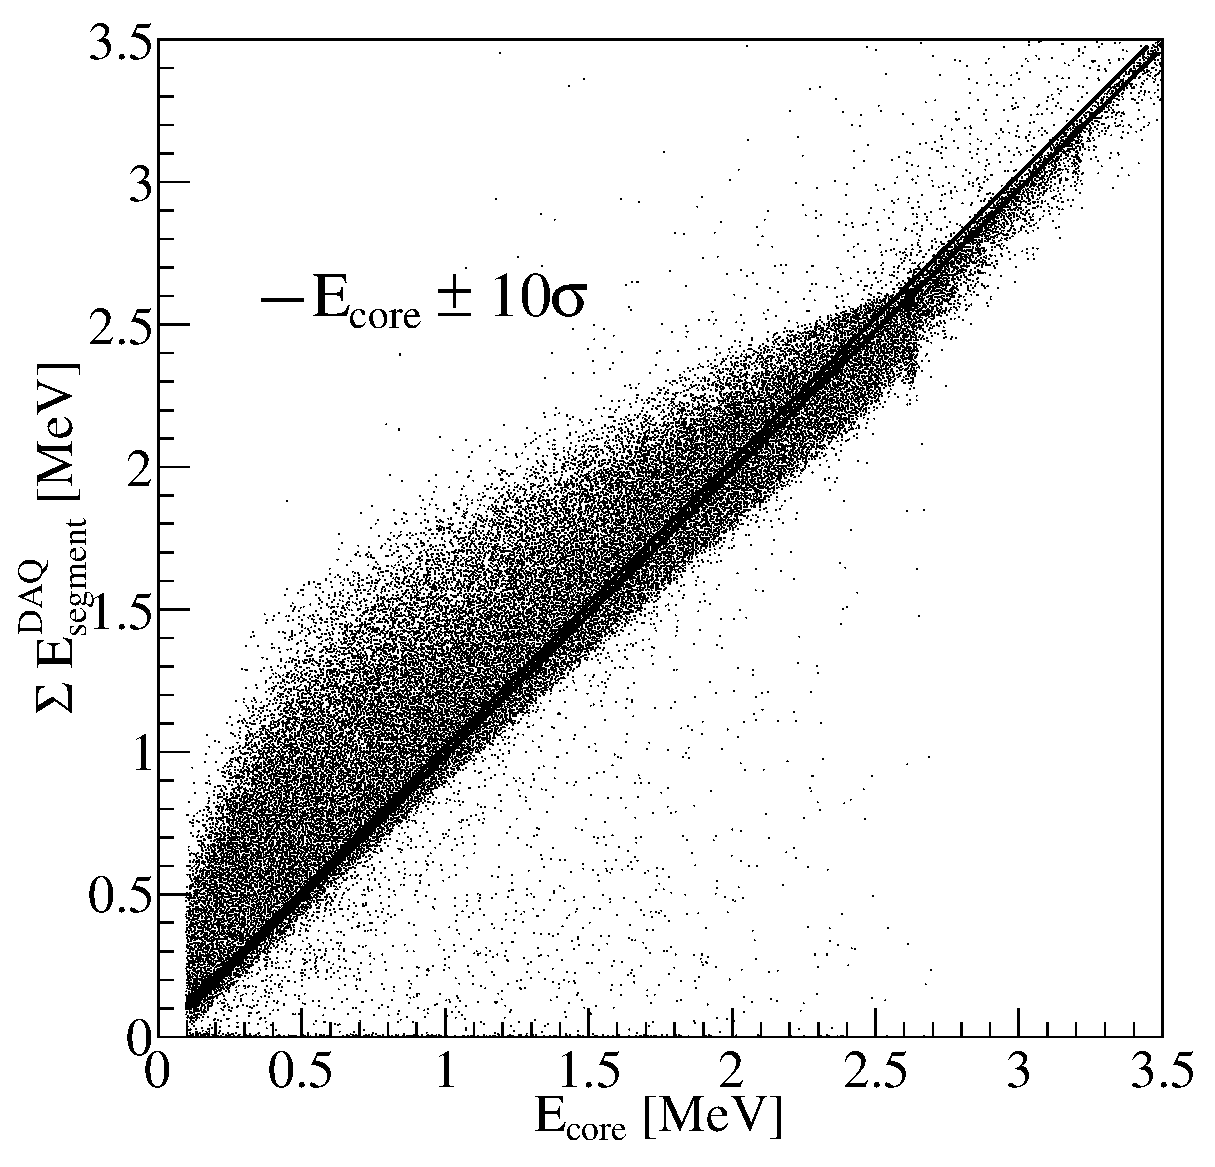
\includegraphics[width=0.5\textwidth]{sEnegPuls}
\caption{Sum of energies from all segments versus the core energy. All energies were calculated by the DAQ system. The two solid lines indicate the 20$\sigma$ range of the core energy.}
\label{fig:ii:sEnegPulse}
\end{figure}

\subsection{Location of negative pulse events}
\label{s:locneg}
To figure out the location of the negative pulse events, the energies from individual segments were plotted versus the core energy as shown in Fig.~\ref{f:ii:EnegPulse}. The two solid lines in the plot indicate the 20$\sigma$ range of the core energy. Negative pulse events were featured with  $E_{\text{segments}} > E_{\text{core}}$. They mainly populated in the segments on the top and bottom of the detector. Very few negative pulse events were found in the segments in the middle of the detector.

\begin{sidewaysfigure}[tphb]
\centering
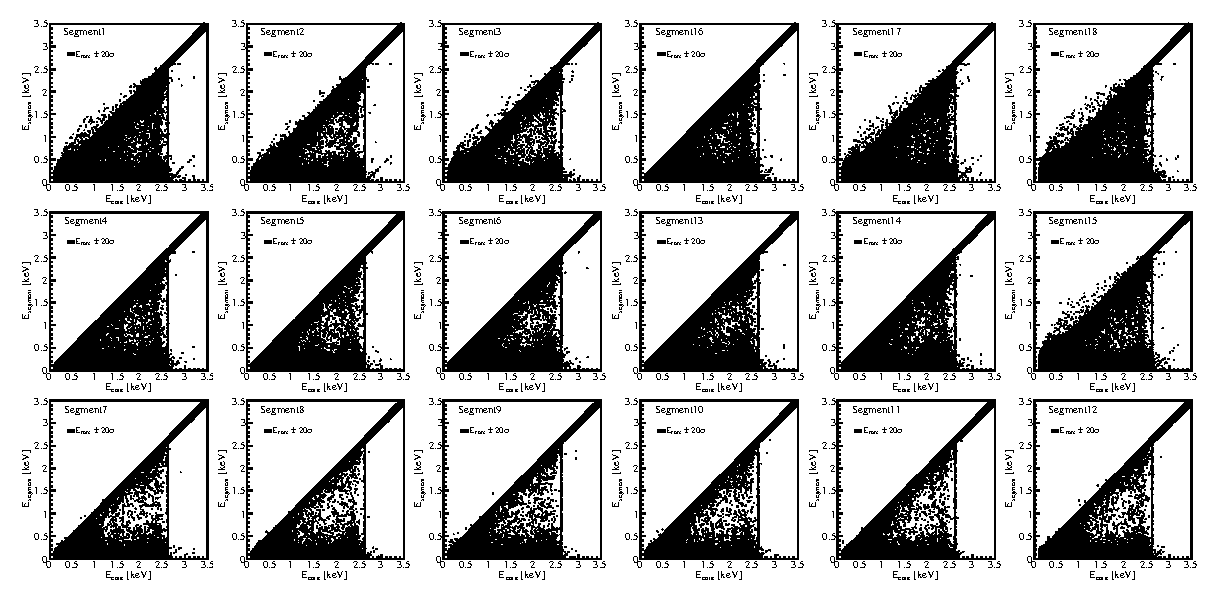
\includegraphics{EnegPuls}
\caption{Energies of individual segments versus the core energy. All energies were calculated by the DAQ system. The two solid lines in each plot indicate the 20$\sigma$ range of the core energy.}
\label{f:ii:EnegPulse}
\end{sidewaysfigure}

\subsection{Possible explanation}
\label{s:ii:exp}
The fact that the negative pulse events populated mainly in the top and bottom segments of the detector indicates that there might be surface channels~\cite{Sur05} formed, where the electric field was distorted and the rise time of the pulse increased subsequently. The DAQ energy filter could not handle the pulse with long rise time correctly and give an energy slightly smaller than the full energy. This would enhance the event rate on the low energy side of a full-energy peak at the cost of the peak itself. This was seen in Fig.~\ref{fig:ph:mca}: the low energy side of the 1332~keV peak in data is significantly higher than that in simulation in which the surface channel effect was not taken into account.

However, if the assumption was true, the fraction of negative pulse events in the low energy photon peaks should be larger than the fraction in the high energy photon peaks. Because low energy photons have a higher probability of depositing their energies close to the detector surface, while photons with higher energy are expected to penetrate deeper into the detector. Events within six photon peaks from the $^{228}$Th energy spectrum were selected to examinate the assumption. They are 239~keV from $^{212}$Pb, 583~keV from $^{208}$Tl, 861~keV from $^{208}$Tl, 2615~keV from $^{208}$Tl and its double- and single-escape peak 1592~keV and 2103~keV. For each of these 6 sub data samples the fractions of events with $\sum E_{\text{segment}} - E_{\text{core}} \gtrsim 20\sigma$ were calculated and plotted as a function of the core energy, as shown in Fig.~\ref{f:fnp_e}. No obvious correlation was found. The assumption hence needs to be studied further more. 

\begin{figure}[tphb]
\centering
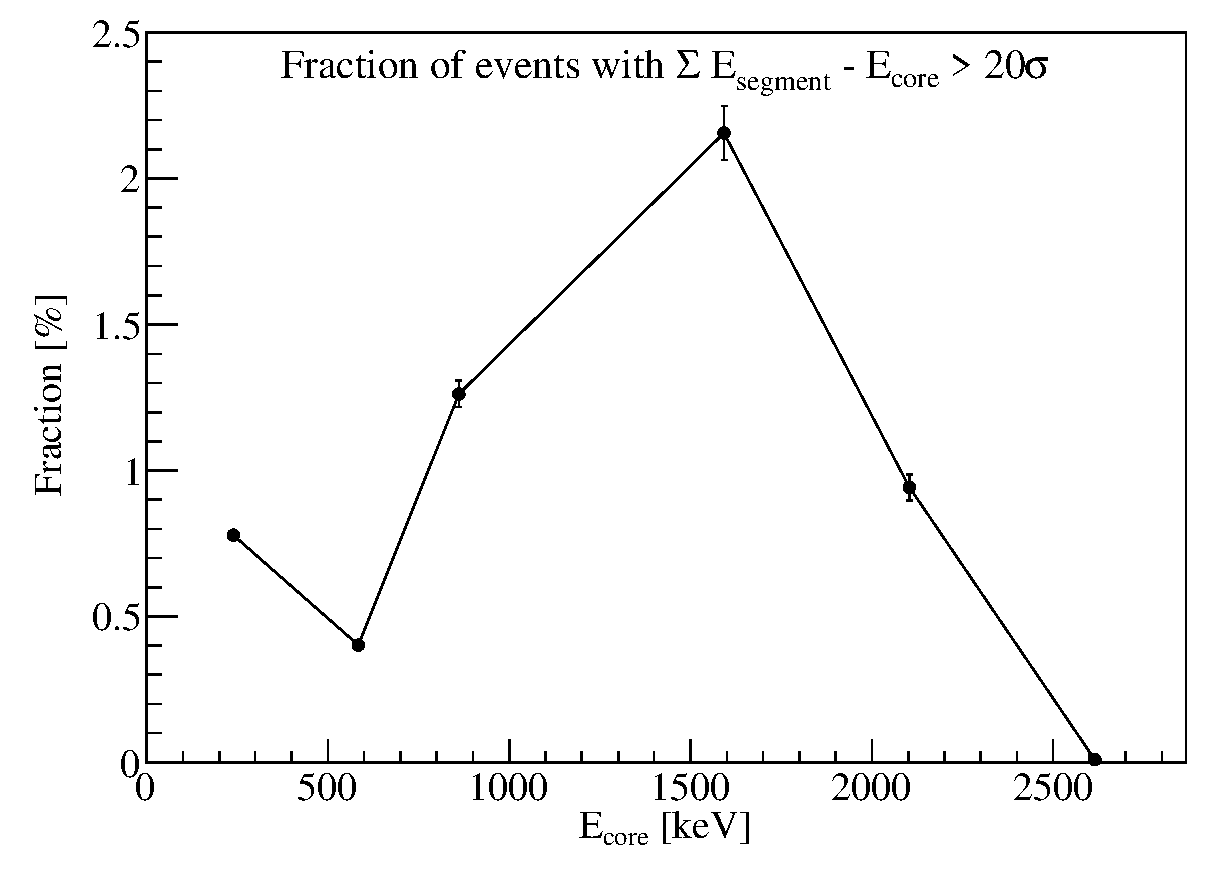
\includegraphics[width=0.6\textwidth]{fnp_e}
\caption{Fraction of events with $\sum E_{\text{segment}} - E_{\text{core}} \gtrsim 20\sigma$ as a function of core energy.}
\label{f:fnp_e}
\end{figure}

\section{Summary}
\label{sec:ii:sum}
A long term operation of Siegfried II directly in liquid nitrogen was performed using GII. Main performance parameters, such as resolution and leakage current, etc., were constantly monitored. Siegfried I was inserted into GII after the first warming-up of Siegfried II. They went through four cooling-down and warming-up cycles together. No obvious decrease of the performance was found. A small fraction of events taken with this setup were found to have negative pulses. Possible explanations were examined. Further investigation are needed.


%%% Local Variables:
%%% mode:latex
%%% TeX-master: "thesis"
%%% End:
